%%%%%%%%%%%%%%%%%%%%%%%%%%%%%%%%%%%%%%%%%%%%%%%%%%%
%
%  New template code for TAMU Theses and Dissertations starting Fall 2016.
%
%
%  Author: Sean Zachary Roberson
%  Version 3.17.09
%  Last Updated: 9/21/2017
%
%%%%%%%%%%%%%%%%%%%%%%%%%%%%%%%%%%%%%%%%%%%%%%%%%%%
%%%%%%%%%%%%%%%%%%%%%%%%%%%%%%%%%%%%%%%%%%%%%%%%%%%%%%%%%%%%%%%%%%%%%%
%%                           TIME TO SOLUTION ESTIMATOR CHAPTER
%%%%%%%%%%%%%%%%%%%%%%%%%%%%%%%%%%%%%%%%%%%%%%%%%%%%%%%%%%%%%%%%%%%%%



\chapter{PARTITIONING OPTIMIZATION \label{cha:optimization}}
In Chapter \ref{cha:tts}, we have seen that we can estimate the time-to-solution for a sweep for different partitioning schemes.
We use the time-to-solution estimator as the objective function in two optimization methods.
The first optimization method utilizes scipy's optimize library, and the second method utilizes knowledge of a problem's mesh layout to assist in partition placement.
%%%%%%%%%%%%%%%%%%%%%%%%%%%%
\section{Scipy optimize}
The scipy optimize library \cite{scipy} provides many tools for optimizing an input function with local and global minimization techniques.
Our usage of the optimize library relies on the minimize function, using the basinhopping \cite{basinhoppingwales} method as the global optimizer, and the constrained Nelder-Mead method as the local optimizer.
We need a global optimization method for larger problem spaces to ensure that cut planes/lines are getting optimized over the entirety of the problem domain, rather than just moving the cut planes/lines close to our initial guess.

The black box tools of scipy optimize are too dependent on the smoothness of the function being optimized.
The time-to-solution estimator is not easily differentiable, and therefore not a smooth enough function even for the parameter spaces of a domain decomposed into 3 subsets in each dimension.
Although utilizing a tested and documented optimizer would have been ideal, it is clear that we need a method more uniquely suited for our problem.

\section{CDF Optimization}

The ``black box'' method using scipy optimize's basinhopping and constrained Nelder-Mead minimizers crashes except for very small parameter spaces.
However, even with modestly large parameter spaces such as the one seen in the Level-2 experiment (Fig. \ref{level2_nocut}), the time-to-solution estimator function is not smooth enough for scipy optimize to honor the constraints or bounds of the problem, leading to the time-to-solution estimator crashing.
This lead to the development of an alternative method, the CDF optimization method.

The CDF optimization method utilizes the geometrical information of the problem to attempt to find optimal cuts. This method prioritizes finding cut line locations that cut along a ``natural boundary'', and minimizing the total number of times the time-to-solution estimator needs to be run.
The time-to-solution estimator for moderately sized problems (such as the Level-2 experiment) can take up to 20 seconds to run for one set of partitions.
This rules out a brute force method of running every possible set of partitions.
Instead, we select our cut lines from the natural boundaries of the mesh.

A natural boundary is a subset boundary that coincides with the geometrical features of the mesh. In Fig.~\ref{natural_boundary_example}, we notice natural boundaries every centimeter in each dimension.
 \begin{figure}[h]
\centering
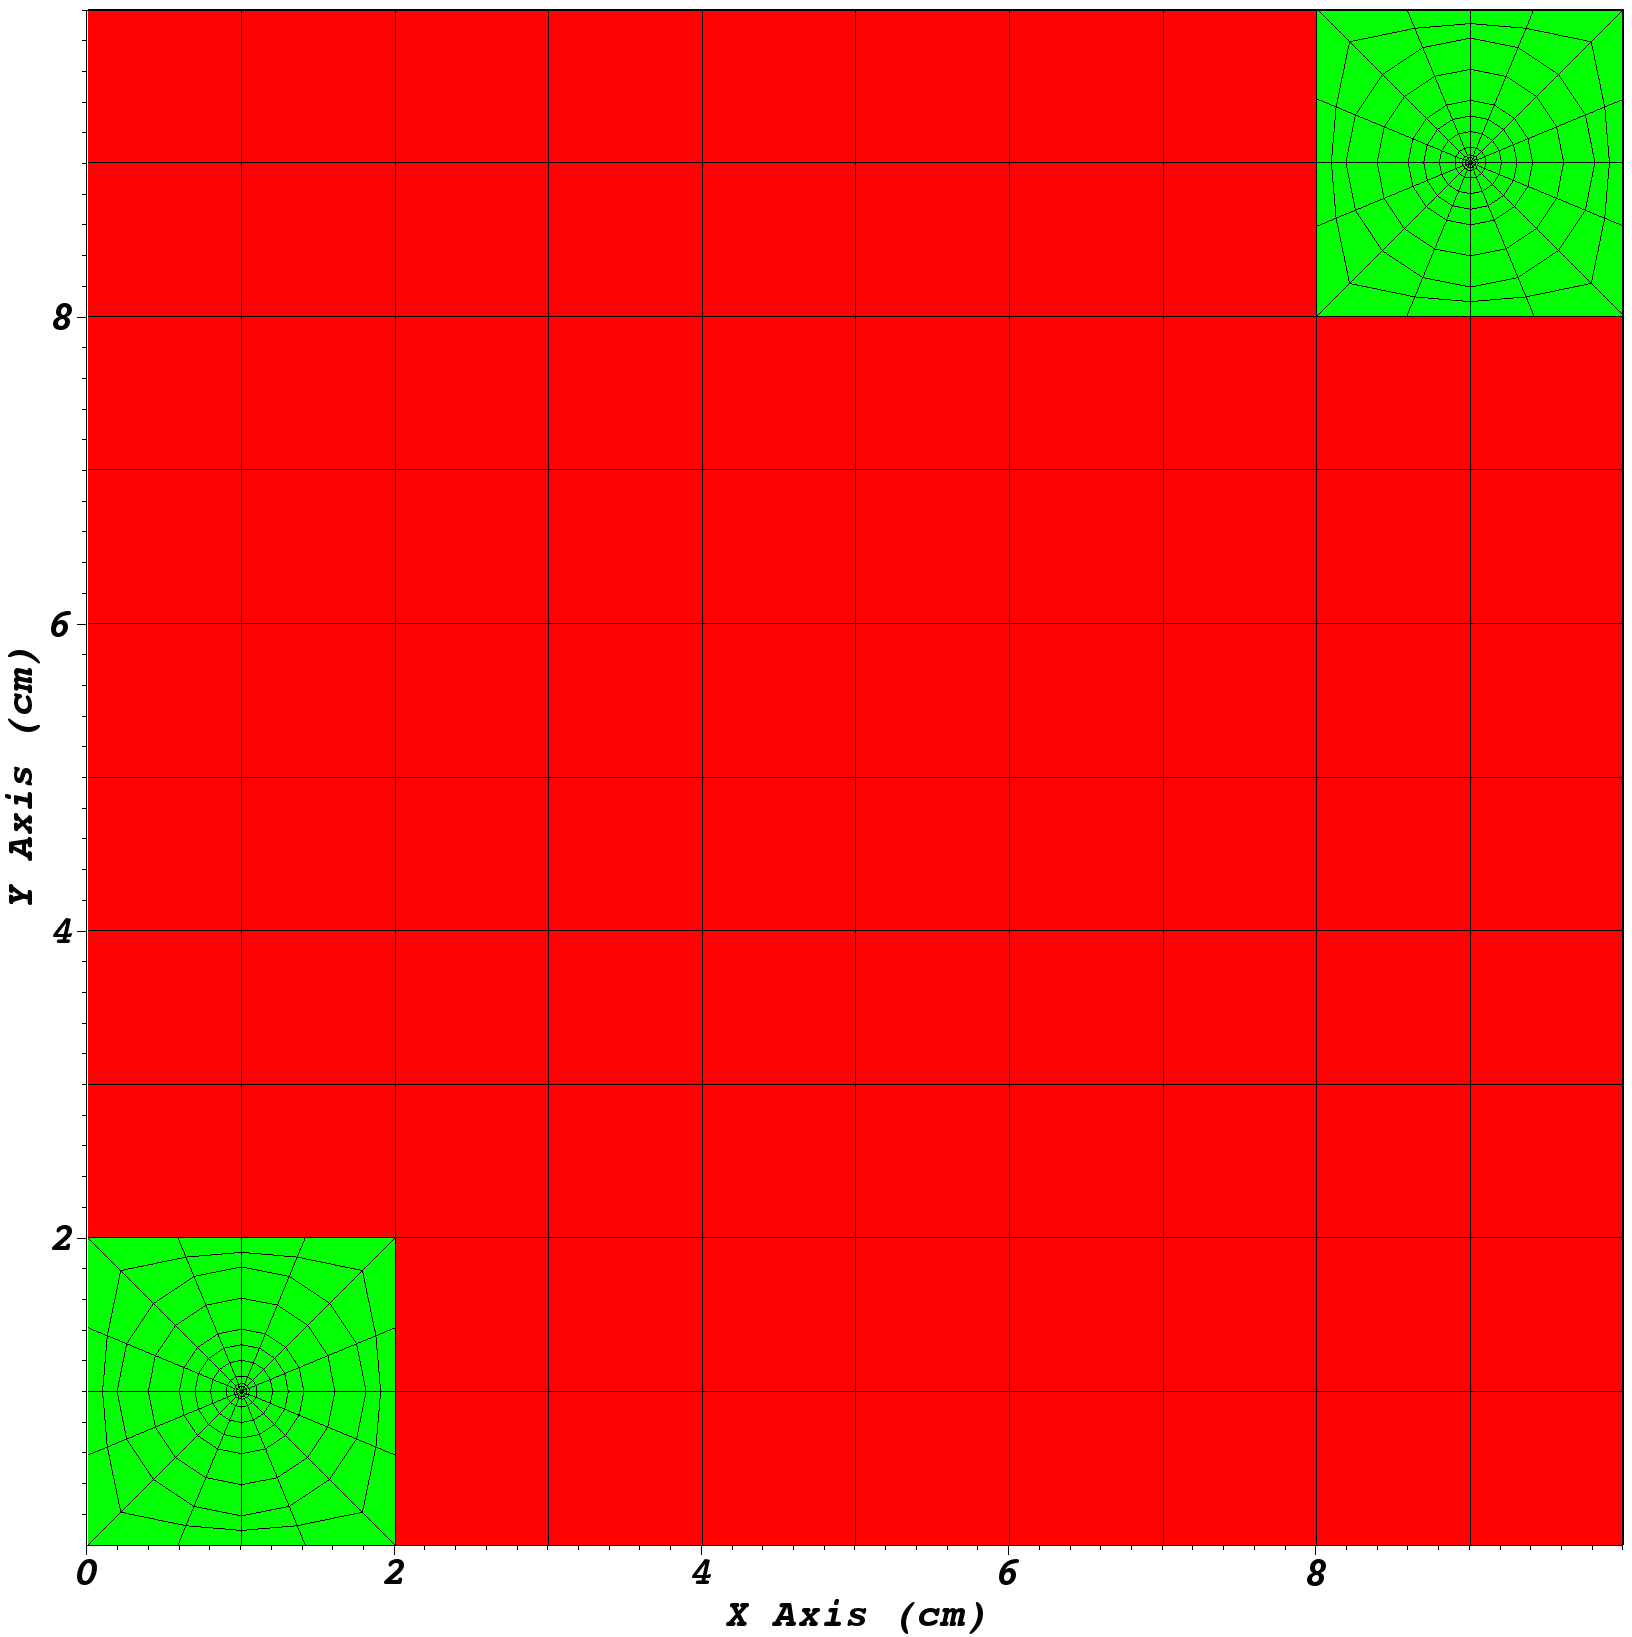
\includegraphics[scale=0.2]{../figures/spiderweb_10x10_sparse.png}
\caption{An unstructured mesh with natural boundaries at 1 cm intervals in both dimensions.}
\label{natural_boundary_example}
\end{figure}

The CDF optimization method will:
\begin{enumerate}
  \item Find the most suitable natural boundaries in the $x$ dimension,
  \item For each set of columns, find the most suitable natural boundaries in the $y$ dimension,
  \item Run all iterations of cut lines selected.
\end{enumerate}

\subsection{Finding the Most Suitable Natural Boundaries}

In order to identify natural boundaries, we analyze the detailed cumulative distribution function (CDF) of the vertices in each dimension. The jumps in the CDF correspond to natural boundaries. Figure~\ref{vert_cdf} shows the x-vertex CDF of the mesh in Fig.~\ref{natural_boundary_example}.
\begin{figure}[h]
\centering
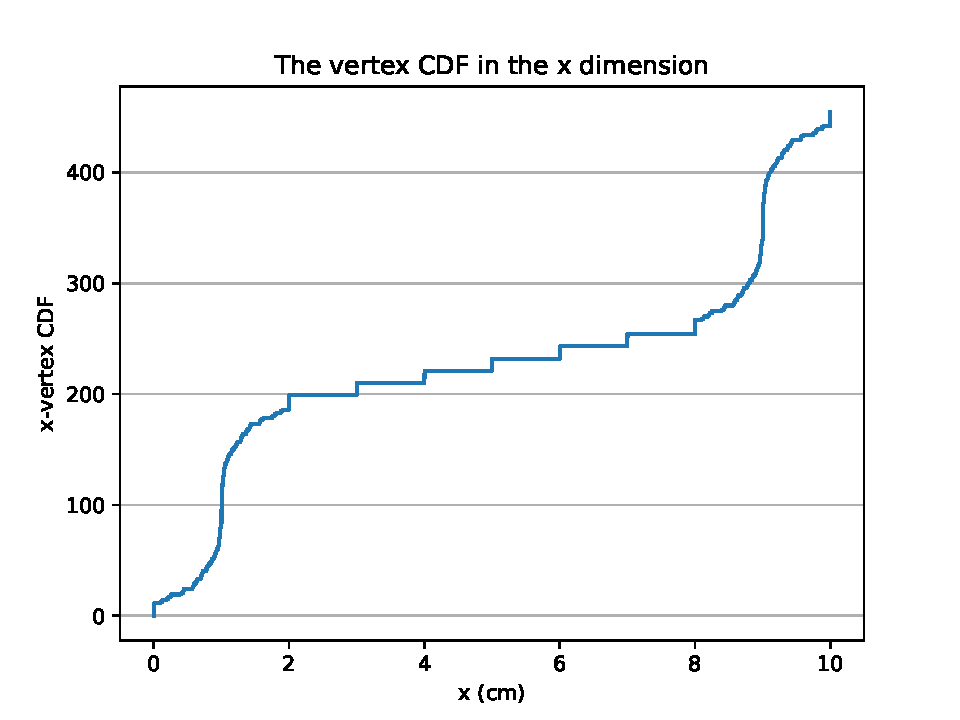
\includegraphics[scale=0.75]{../figures/xvertexcdf.pdf}
\caption{The x-vertex CDF of the mesh shown in Fig.~\ref{natural_boundary_example}}.
\label{vert_cdf}
\end{figure}

To identify where the jumps in the CDF occur, we take the normalized derivative of the CDF and isolate the largest discontinuities in it. Figure~\ref{gradcdf} plots the derivative of the CDF shown in Fig.~\ref{vert_cdf}.
\begin{figure}[h]
\centering
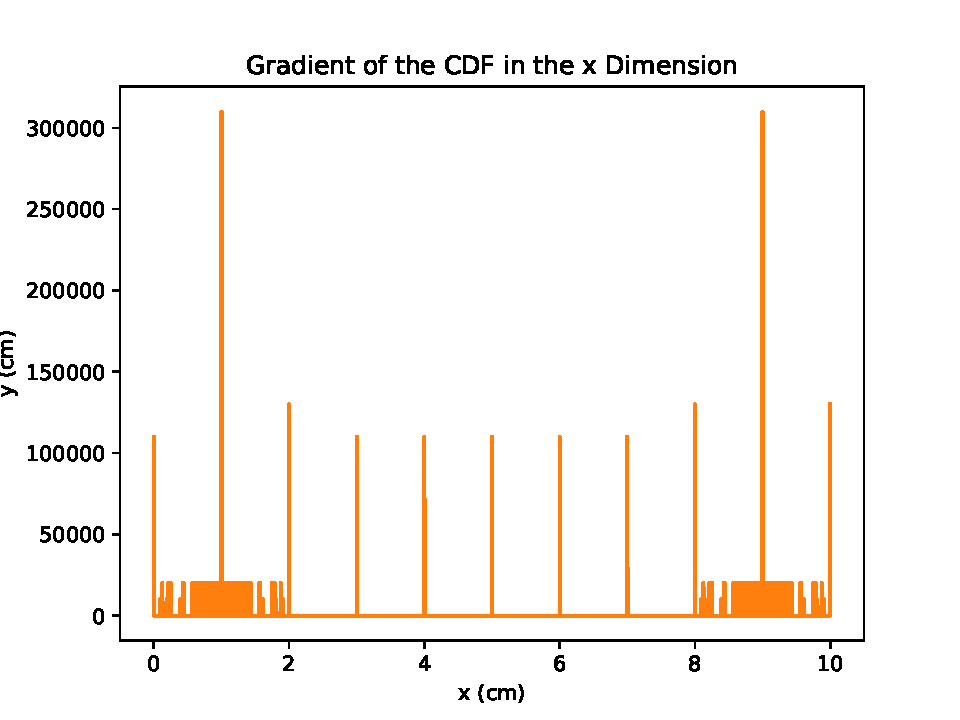
\includegraphics[scale=0.75]{../figures/gradcdf.pdf}
\caption{The derivative of the CDF shown in Fig.~\ref{vert_cdf}.}
\label{gradcdf}
\end{figure}
The largest discontinuities in Fig.~\ref{gradcdf} occur at the instances where there are natural boundaries all the way through the mesh, or at 1 cm intervals.
We should note that although the global boundaries of the problem have discontinuities, these discontinuities are obviously not eligible to be chosen as potential partitions.

The process to select the most suitable natural boundaries occurs in two steps.
The first step is to to choose cuts that balance the number of vertices per dimension.
This is done by finding the intersection of the CDF with an ideal number of vertices per partition, similar to what the redistribution function in the load balancing algorithms does in Fig.~\ref{redistribute}.
Instead of using the cells per dimension CDF, we use the vertex per dimension CDF of Fig.~\ref{vert_cdf}.

Once we have the cuts that balance the vertices of the mesh, we wish to move the cuts to locations that minimize the additions of cells to the mesh.
For each balanced cut, we ``snap'' it to a location corresponding to a natural boundary.
We explored choosing where to snap the cut to in one of two ways:
\begin{enumerate}
  \item Snapping the balanced cuts to the largest discontinuities in the derivative of the CDF.
  \item Snapping the balanced cut to a discontinuity that takes into account how close a discontinuity is, as well as the magnitude of the discontinuity.
\end{enumerate}

The first snapping method does not take into account the location of the balanced cuts, and instead just chooses the largest discontinuities in the derivative of the CDF.

The second and third methods choose where to snap each balanced cut based on the distance of the balanced cuts from nearby natural boundaries. Eq.~\ref{distance} shows the calculation of the smallest weighted distance:
\begin{equation}
d = \underset{i \in \text{pool}}{\text{min}} \frac{|x^{*} - x_i|}{J_i}
\label{distance}
\end{equation}
where $d$ is the smallest weighted distance, $x^*$ is a balanced cut, $x_i$ is a natural boundary we are testing, and $J_i$ is the magnitude of the normalized derivative corresponding to $x_i$.
The \text{pool} is a subset of the discontinuities in the derivative of the CDF.
Rather than test against every possible natural boundary, we pull a subset of discontinuities whose magnitudes are over a certain value.
This prevents from unnecessarily testing small jumps that only have natural boundaries through a very small portion of the mesh.

\FloatBarrier
\subsection{Finding Natural Boundaries for Sets of Columns}
In order to globalize the optimization of the cut lines per column, we set up a binary tree of test cases, such as the one shown in Fig.~\ref{binary_tree}. Each layer in the tree represents one set of $y$ cut lines. The first layer, or the root of the tree, represents the case where we try and find the natural boundaries in $y$ throughout all columns, in this case 4 columns. The next layer tries to find two sets of natural boundaries, one set of natural $y$ boundaries through the first two columns, and another set through the final 2 columns. Finally, the last case finds a set of natural $y$ boundaries in each individual column.

\begin{figure}[h]
\centering
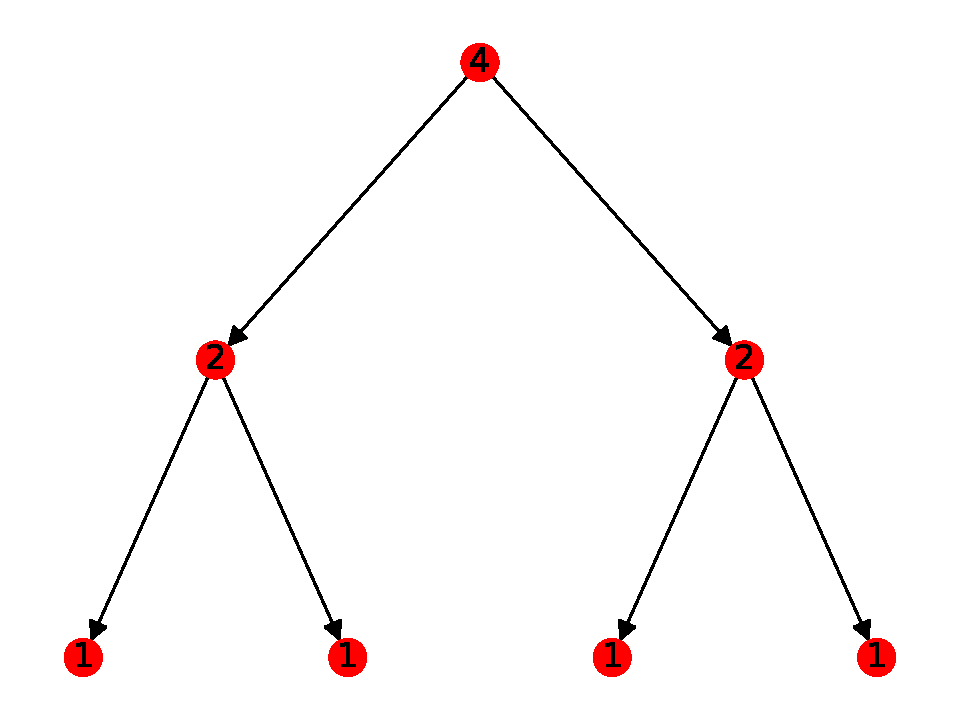
\includegraphics[scale=0.75]{../figures/binary_tree.pdf}
\caption{A binary tree where each node represents the number of columns we are attempting to find a natural boundary through.}
\label{binary_tree}
\end{figure}

Let us consider the mesh of the Level-2 experiment shown in Fig.~\ref{level2_nocut}.
We run this problem with 42 subsets in $x$ and 13 subsets in $y$.
Fig.~\ref{opt_walkthrough} shows 3 stages of choosing partitions for the Level-2 mesh.
Fig.~\ref{42} shows the $x$ partitions, with the $y$ partitions optimized for all 42 columns.
This means that we attempted to identify natural boundaries through all 42 columns.
Fig.~\ref{21} shows the same $x$ partitions, but the $y$ partitions optimized for the first 21 columns independently from the second 21 columns.
Fig.~\ref{10} shows the same $x$ partitions, with the $y$ partitions optimized independently for first 10 columns, then the next 11 columns, then the next 10 columns, then the next 11 columns.
We continue this process until we are optimizing $y$ partitions for each column.
%%%%%%%%%%%%%%%
\begin{figure}[h]
\centering
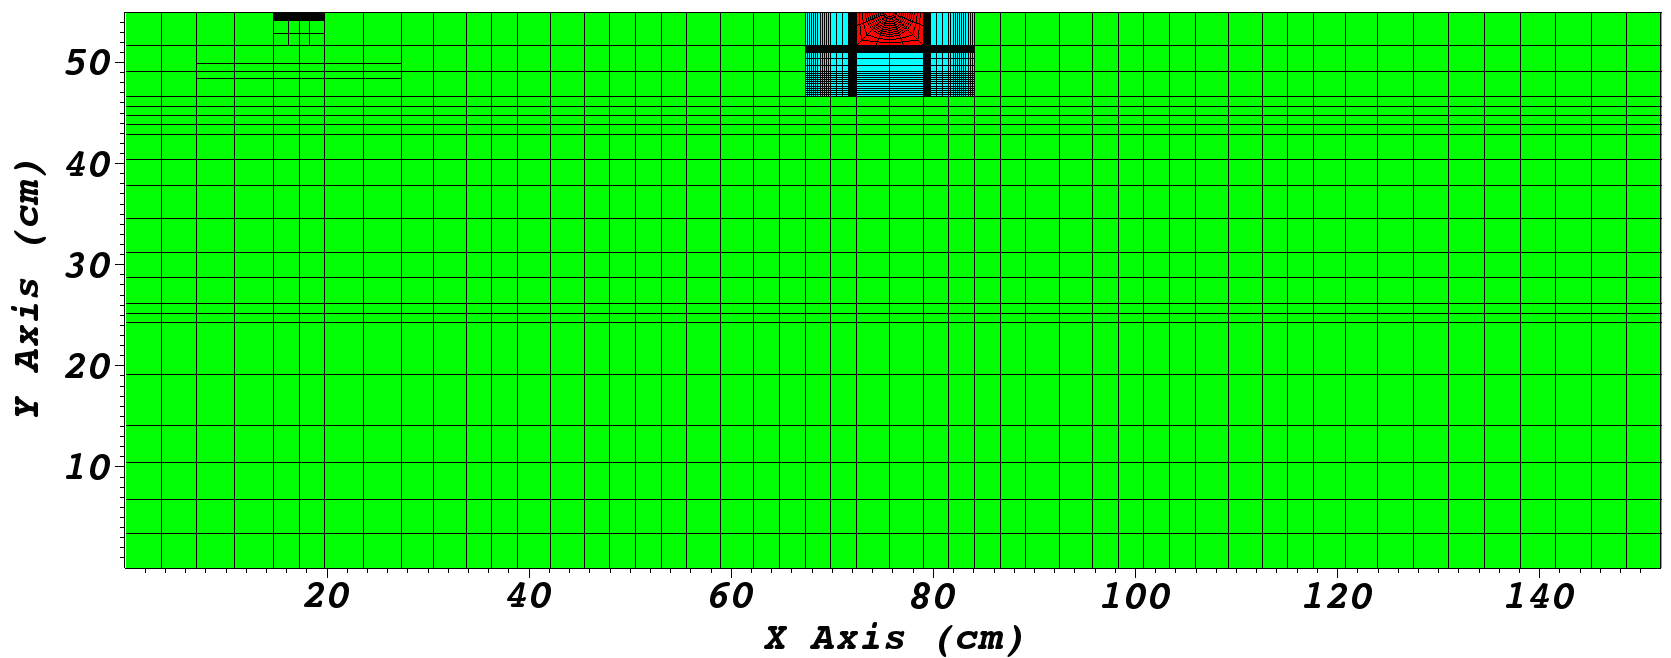
\includegraphics[scale=0.3]{../../figures/level2_nocut.png}
\caption{The mesh for the Level-2 experiment.}
\label{level2_nocut}
\end{figure}

\begin{figure}[h]
\centering
  \begin{subfigure}[t]{\textwidth}
    \centering
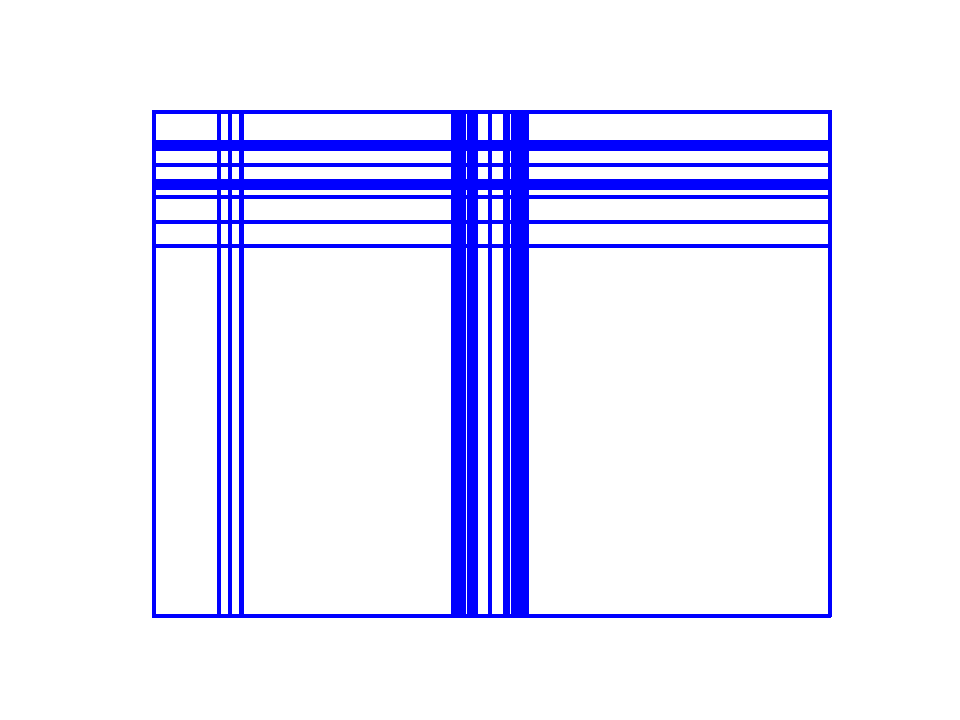
\includegraphics[scale=0.5]{../../figures/lvl2_suite_0.pdf}
  \caption{The y-cuts chosen for all 42 columns.}
    \label{42}
  \end{subfigure}
  \begin{subfigure}[b]{\textwidth}
    \centering
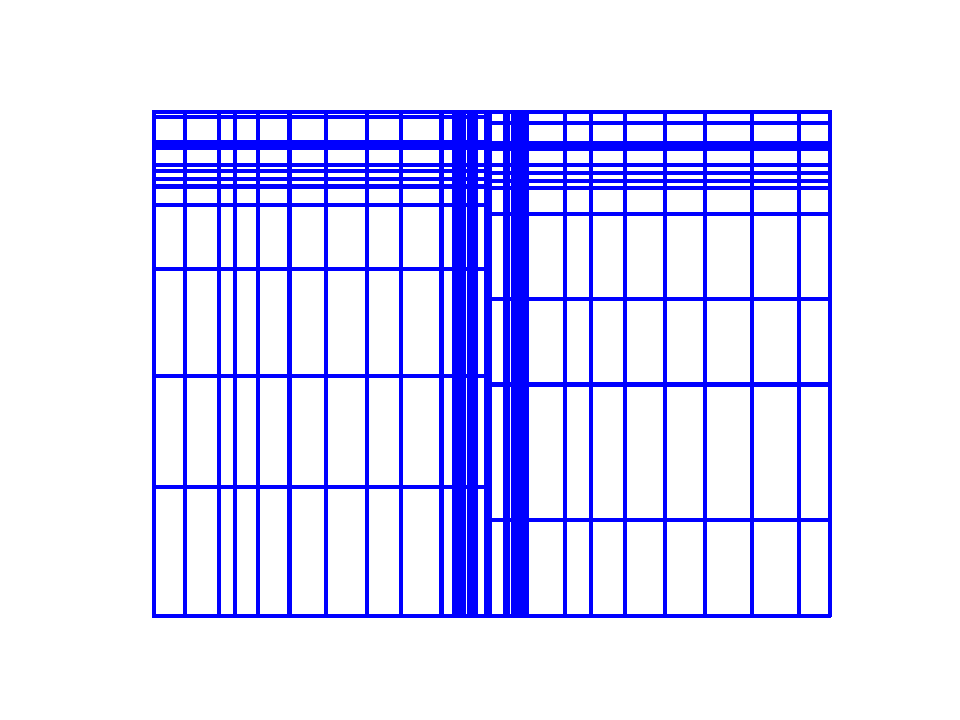
\includegraphics[scale=0.5]{../../figures/lvl2_suite_1.pdf}
    \caption{The y-cuts chosen independently for the first 21 columns and the second 21 columns}.
    \label{21}
  \end{subfigure}
  \begin{subfigure}[b]{\textwidth}
    \centering
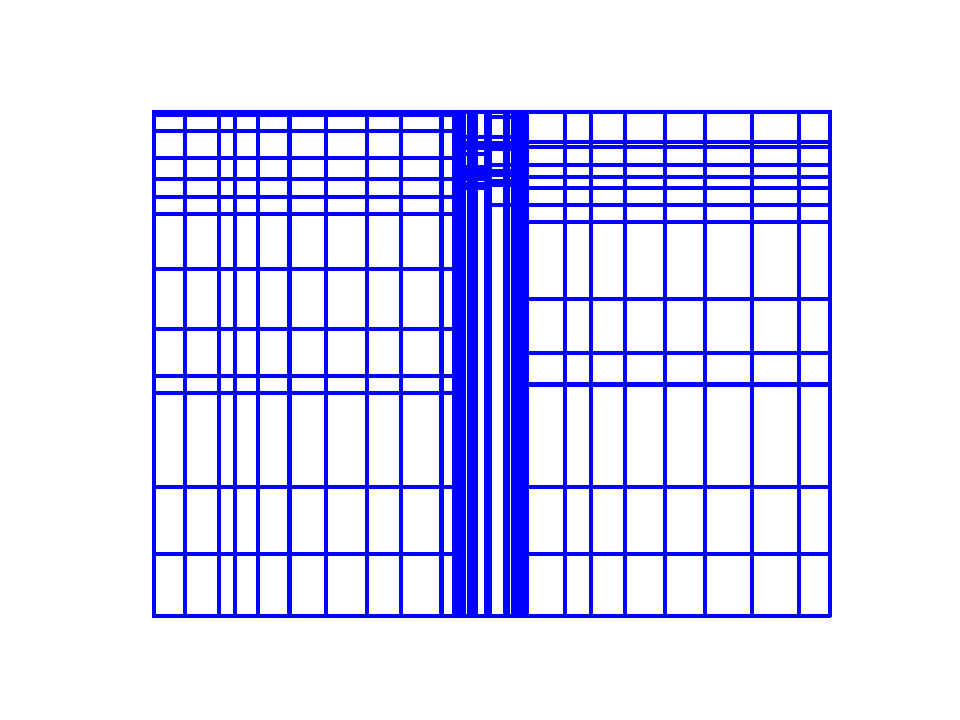
\includegraphics[scale=0.5]{../../figures/lvl2_suite_2.pdf}
    \caption{The y-cuts chosen independently for 10,11,10, and 11 columns.}
    \label{10}
  \end{subfigure}
  \caption{The Level-2 Mesh partitions at three stages of the choosing the optimization cut process.}
  \label{opt_walkthrough}
\end{figure}

This method of optimization allows us to select a set of partitions with an attempt to optimize over the global domain.
With this method, we are also not running the time-to-solution estimator a large number of times, instead electing to using use it in an intuitive automation process.

\FloatBarrier

\section{Optimization Results}

The results reported utilize the second ``snapping'' method, where cuts are snapped to a discontinuity that takes into account how close a discontinuity is, as well as the magnitude of the discontinuity.
This method always outperformed the first method of snapping cuts to the largest discontinuities in the derivative of the CDF.

The CDF optimization method was run on the unbalanced pin mesh and the Level-2 experiment mesh.
The unbalanced pin mesh was run through the optimization suite from 2 to 10 subsets in each dimension.
Figure~\ref{ubp_opt} shows the time-to-solution for binary tree, regular, load-balanced and load-balanced-by-dimension cuts on the unbalanced pins mesh from 2 to 10 subsets in each dimension.
%%%%%%%%%%
\begin{figure}[ht]
\centering
  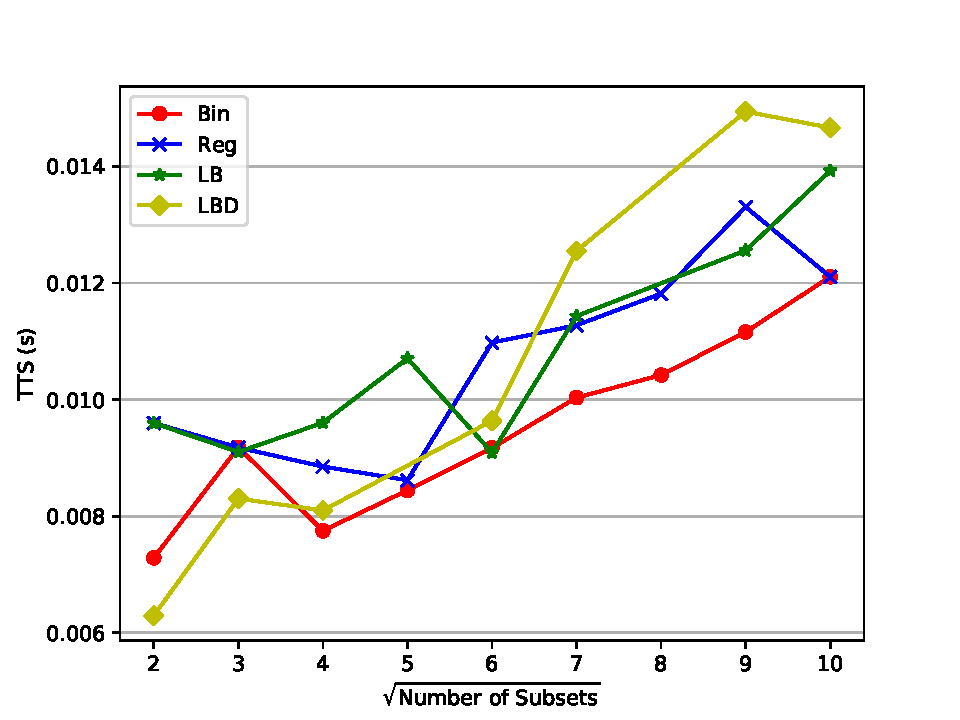
\includegraphics{../../figures/unbalanced_pins_best_comparison.pdf}
  \caption{The time-to-solution for binary tree, regular, load-balanced and load-balanced-by-dimension cuts on the unbalanced pins mesh from 2 to 10 subsets in each dimension.}
  \label{ubp_opt}
\end{figure}
%%%%%%%%%%%
For low numbers of subsets, the load-balanced-by-dimension partitions outperform the regular, load-balanced, and optimized partitions.
Due to the low number of communications, having partitions that are balanced by column does not incur a large communication penalty, and having a well-balanced problem is still more important.
However, once we exceed 9 subsets, we can see the optimized partitions outperforming the other partition types, with the prioritization of not adding cells paying off.

Figure~\ref{ubp_opt_heavy} shows the time-to-solution for binary tree, regular, load-balanced and load-balanced-by-dimension cuts on the ``heavier'' unbalanced pins mesh from 2 to 10 subsets in each dimension.
\begin{figure}[ht]
\centering
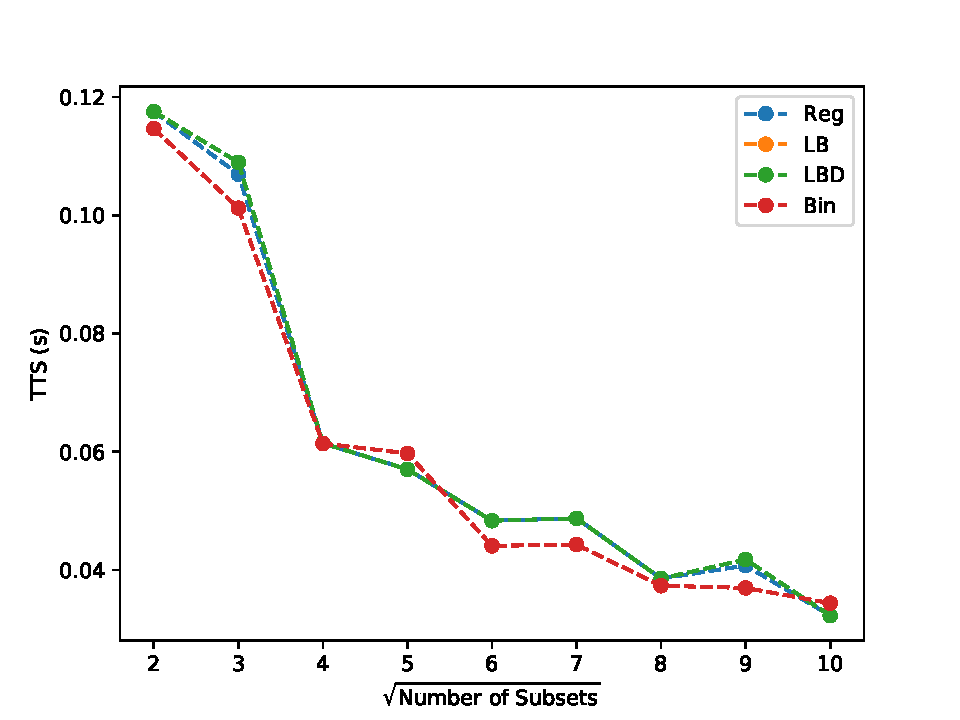
\includegraphics{../../figures/more_sparse_best_comp.pdf}
  \caption{The time-to-solution for binary tree, regular, load-balanced and load-balanced-by-dimension cuts on the ``heavier'' unbalanced pins mesh from 2 to 10 subsets in each dimension.}
  \label{ubp_opt_heavy}
\end{figure}
%%
For the majority of cases run with this mesh, the binary tree cuts outperform the regular, load-balanced, and load-balanced-by-dimension cuts.

Figure~\ref{level2_opt} shows the sweep times on the Level-2 mesh from the time-to-solution estimator and PDT for (1) regular cuts, (2) hand-balanced cuts, (3) load-balanced cuts, (4) load-balanced-by-dimension cuts, and (5) binary tree cuts.
\begin{figure}[ht]
\centering
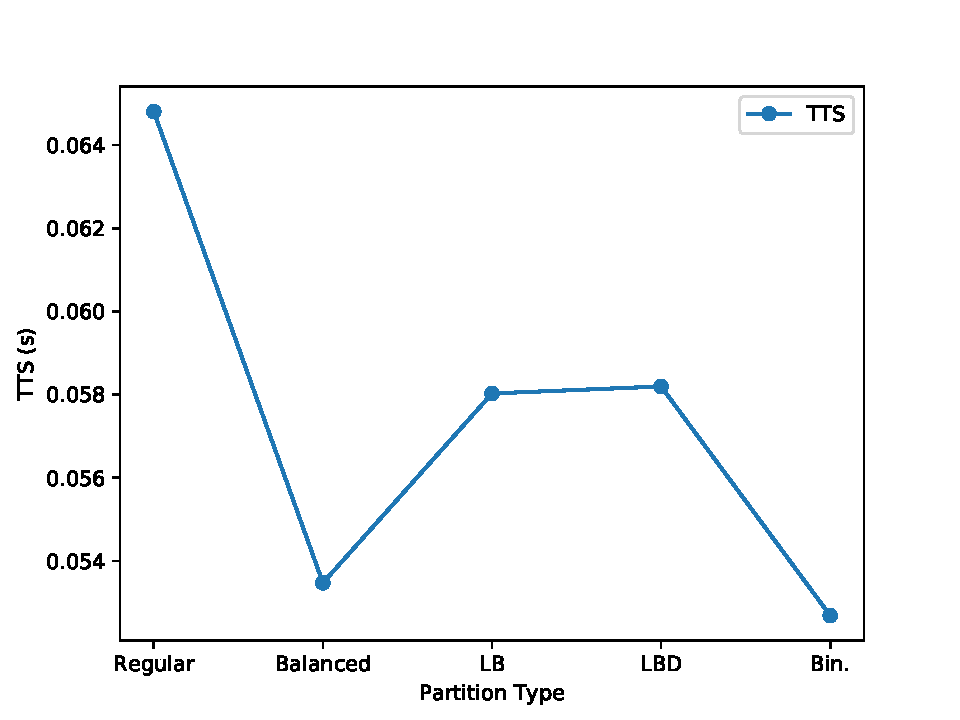
\includegraphics{../../figures/level2_sweep_comp_best.pdf}
\caption{The Level-2 mesh sweep times from the time-to-solution estimator for (1) regular cuts, (2) hand-balanced cuts, (3) load-balanced cuts, (4) load-balanced-by-dimension cuts, and (5) optimized cuts. }
\label{level2_opt}
\end{figure}
The time to solution of the binary tree cuts is 1.5\% better than the hand-balanced cuts.
The binary cut suite for the Level-2 experiment mesh took about 2 minutes to find the minimum time to solution, while hand-balancing the mesh took at least an hour.
Even though 1.5\% may seem like a negligible difference, the difference in time spent to get a similar time-to-solution should be taken into account and highlight the significance of the improvement.

Figure~\ref{im1c_opt} shows the results of the IM1C experiment mesh run through the time-to-solution estimator for regular, load-balanced-by-dimension, and binary tree cuts with 5 subsets in each dimension.
\begin{figure}[ht]
\begin{minipage}[c]{0.65\textwidth}
\centering
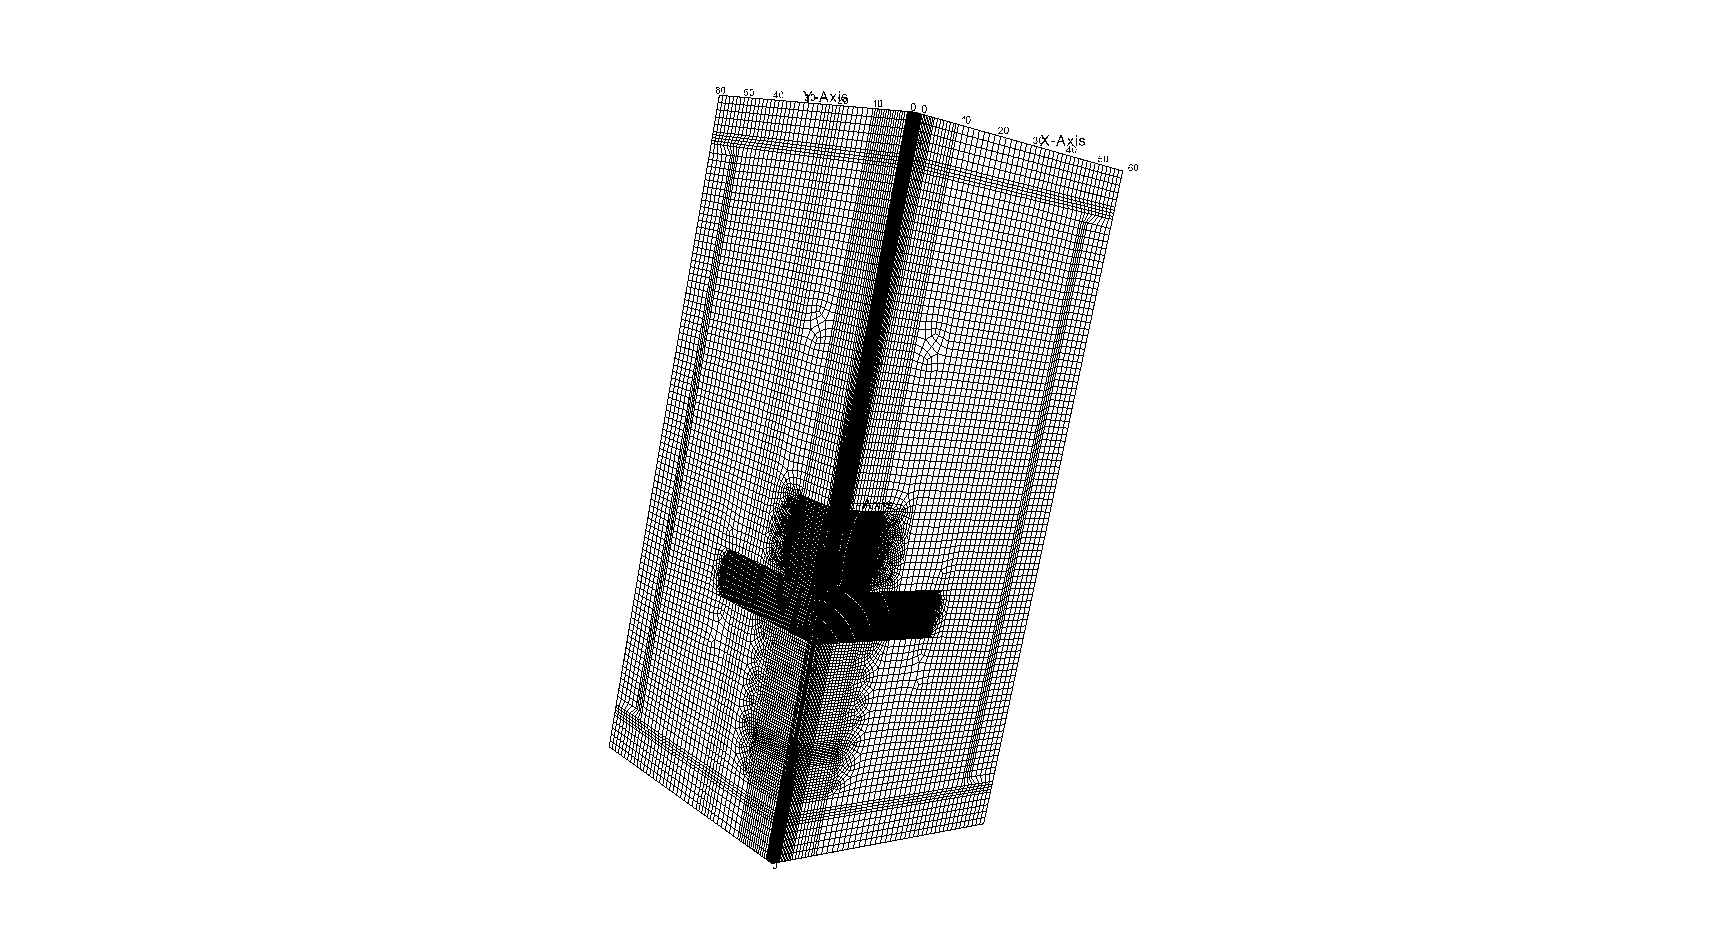
\includegraphics[scale=0.3]{../figures/im1_mesh.png}
\end{minipage}
%
\begin{minipage}[c]{0.33\textwidth}
\centering
\begin{table}[H]
\centering
\begin{tabular}{c|c|c}
\textbf{Type} & \bf TTS (s) & \bf $f$ \\ \hline
Regular & 3.804 & 12.329\\ \hline
LBD & 1.836 & 1.008\\ \hline
Bin. & 0.926 & 1.918\\ \hline
\end{tabular}
\end{table}
\end{minipage}
\caption{The IM1C experiment mesh run through the time-to-solution estimator for regular, load-balanced-by-dimension, and binary tree cuts with 5 subsets in each dimension. Additionally, the load-balance metric $f$ is reported for each partition type.}
\label{im1c_opt}
\end{figure}
The binary tree cuts beat both the regular and load-balanced-by-dimension cuts by a large margin. In addition, the load-balancing data shows that just because a problem is more balanced, even by a large margin, does not mean the time-to-solution is better.

The CDF optimization method provides a partitioning scheme with a time-to-solution that is better than regular, load-balanced, and load-balanced-by-dimension partitions for the majority of cases run.
Choosing cuts that balance the vertices by dimension followed by snapping those cuts to locations less likely to add cells to the mesh proves to be quite effective.

However, we two paths forward for improvement come to mind.
With a sped up time-to-solution estimator, we can run several more possible sets of partitions.
For example, combinations of natural boundaries could be run rather than choosing the most suitable every time.

Additionally, exploring different formulations for Eq.~\ref{distance}, or the calculation of the smallest weighted distance, could yield interesting results.

